\documentclass[11pt]{article}
\usepackage{geometry}
\geometry{margin=1in}
\usepackage{graphicx}
\usepackage{hyperref}
\usepackage{amsmath}
\usepackage{tikz}
\usetikzlibrary{arrows.meta, positioning, shapes.multipart}
\title{\textbf{XAI-Lab: Technical and Architectural Documentation}}
\author{Generated by GitHub Copilot}
\date{\today}

\begin{document}
\maketitle

\tableofcontents
\newpage

% =====================
\section{Project Overview}
XAI-Lab is a modular, containerized platform for credit risk modeling, explainable AI (XAI), and fairness auditing. It is designed for reproducible ML workflows, model interpretability, and deployment in both Docker Compose and Kubernetes environments.

\subsection{Goals}
\begin{itemize}
  \item Train and evaluate credit risk models with explainability and fairness metrics.
  \item Serve predictions via a REST API (FastAPI backend).
  \item Support multi-dataset, multi-backend deployment (load balancing, hot-reload).
  \item Enable reproducible experiments and MLflow tracking.
  \item Deployable on local machines (Docker Compose) and cloud (Kubernetes).
\end{itemize}

% =====================
\section{High-Level Architecture}
\subsection{Component Diagram}
\begin{center}
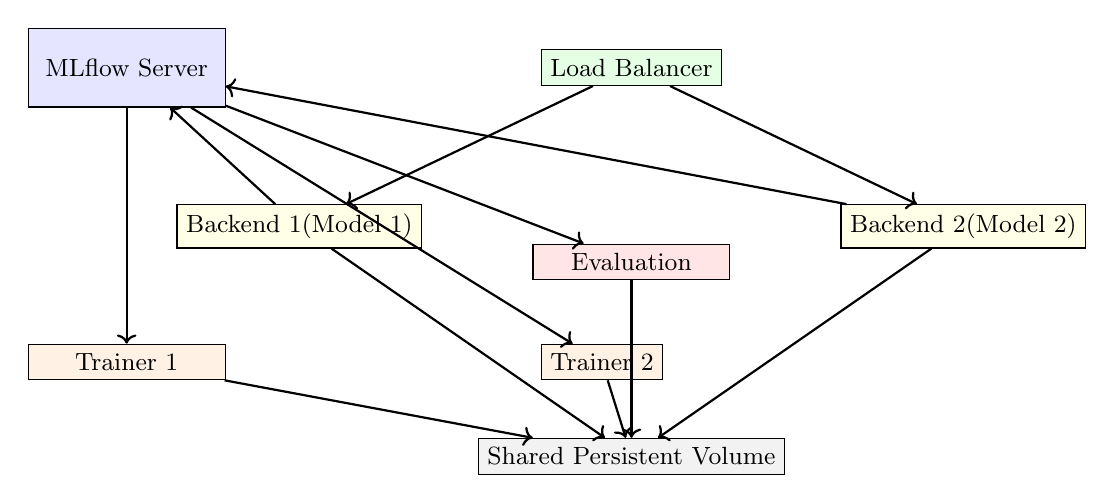
\begin{tikzpicture}[node distance=2.5cm, every node/.style={font=\small}]
  % Nodes
  \node[draw, rectangle, fill=blue!10, minimum width=2.5cm, minimum height=1cm] (mlflow) {MLflow Server};
  \node[draw, rectangle, fill=green!10, right=4cm of mlflow] (lb) {Load Balancer};
  \node[draw, rectangle, fill=yellow!10, below left=1.5cm and 1.5cm of lb] (backend1) {Backend 1\\(Model 1)};
  \node[draw, rectangle, fill=yellow!10, below right=1.5cm and 1.5cm of lb] (backend2) {Backend 2\\(Model 2)};
  \node[draw, rectangle, fill=orange!10, below=3cm of mlflow, minimum width=2.5cm] (trainer1) {Trainer 1};
  \node[draw, rectangle, fill=orange!10, right=4cm of trainer1] (trainer2) {Trainer 2};
  \node[draw, rectangle, fill=red!10, below=2cm of lb, minimum width=2.5cm] (eval) {Evaluation};
  \node[draw, rectangle, fill=gray!10, below=2cm of eval, minimum width=3cm] (pv) {Shared Persistent Volume};
  % Edges
  \draw[->, thick] (lb) -- (backend1);
  \draw[->, thick] (lb) -- (backend2);
  \draw[->, thick] (backend1) -- (pv);
  \draw[->, thick] (backend2) -- (pv);
  \draw[->, thick] (trainer1) -- (pv);
  \draw[->, thick] (trainer2) -- (pv);
  \draw[->, thick] (eval) -- (pv);
  \draw[->, thick] (mlflow) -- (trainer1);
  \draw[->, thick] (mlflow) -- (trainer2);
  \draw[->, thick] (mlflow) -- (eval);
  \draw[->, thick] (backend1) -- (mlflow);
  \draw[->, thick] (backend2) -- (mlflow);
\end{tikzpicture}
\end{center}

\subsection{Service Overview}
\begin{itemize}
  \item \textbf{MLflow Server}: Tracks experiments, metrics, and artifacts.
  \item \textbf{Trainer(s)}: Train XGBoost models on different datasets, save to shared volume.
  \item \textbf{Backend(s)}: Serve predictions via FastAPI, hot-reload models.
  \item \textbf{Load Balancer}: Distributes API requests across backends.
  \item \textbf{Evaluation}: Computes metrics, fairness, and XAI visualizations.
  \item \textbf{Persistent Volume}: Shared storage for models and artifacts.
\end{itemize}

% =====================
\section{Data Flow and Pipeline}
\subsection{Training Pipeline}
\begin{enumerate}
  \item Load dataset (CSV).
  \item Preprocess features (categorical encoding, scaling).
  \item Train XGBoost classifier (with/without gender).
  \item Save pipeline (preprocessor + model) to shared volume.
  \item Log metrics and artifacts to MLflow.
\end{enumerate}

\subsection{Inference Pipeline}
\begin{enumerate}
  \item Backend loads model pipeline from shared volume.
  \item Receives REST API requests (JSON input).
  \item Preprocesses input, predicts risk, returns result.
  \item Supports hot-reload (model file changes).
\end{enumerate}

\subsection{Evaluation Pipeline}
\begin{enumerate}
  \item Loads trained model and test data.
  \item Computes performance metrics (accuracy, F1, ROC, etc.).
  \item Computes fairness metrics (demographic parity, equalized odds).
  \item Generates XAI visualizations (SHAP, LIME).
  \item Saves plots to visualization directory.
\end{enumerate}

% =====================
\section{Component Details}
\subsection{Training (train.py, model_trainer.py)}
\begin{itemize}
  \item Uses \texttt{XGBClassifier} with configurable features.
  \item Handles gender as a protected attribute (fairness analysis).
  \item Saves pipeline as a \texttt{.joblib} file.
  \item Can be run as a script or as a Kubernetes CronJob.
\end{itemize}

\subsection{Inference (inference.py, backend.py)}
\begin{itemize}
  \item FastAPI app exposes /predict endpoint.
  \item Loads model pipeline, preprocesses input, returns prediction.
  \item Backend supports hot-reload and multi-model serving (via env vars).
\end{itemize}

\subsection{Evaluation (evaluate.py)}
\begin{itemize}
  \item Loads model and test data.
  \item Computes confusion matrix, ROC, F1, precision, recall, etc.
  \item Computes fairness metrics using \texttt{fairlearn}.
  \item Generates SHAP and LIME explanations.
  \item Saves all plots to disk.
\end{itemize}

\subsection{Load Balancer (load_balancer.py)}
\begin{itemize}
  \item Flask app forwards requests to backends in round-robin fashion.
  \item Uses environment variables for backend URLs.
  \item Designed for Kubernetes service discovery.
\end{itemize}

\subsection{MLflow Integration (mlflow_logger.py)}
\begin{itemize}
  \item Logs metrics, parameters, and artifacts for each run.
  \item Supports experiment tracking and reproducibility.
\end{itemize}

% =====================
\section{Deployment}
\subsection{Docker Compose}
\begin{itemize}
  \item Compose file defines MLflow, trainers, evaluation, backends, and load balancer.
  \item Volumes are used for sharing models and artifacts.
  \item Services can be scaled and restarted independently.
\end{itemize}

\subsection{Kubernetes}
\begin{itemize}
  \item Manifests define PersistentVolumeClaim, CronJobs (trainers), Deployments (backends, load balancer), and Services.
  \item Trainers write models to shared volume; backends hot-reload.
  \item Load balancer uses ClusterIP service names for backend discovery.
\end{itemize}

% =====================
\section{Extending and Modifying the System}
\subsection{Adding New Features}
\begin{itemize}
  \item \textbf{New Model Types}: Add new trainers or modify \texttt{train.py} to use different algorithms.
  \item \textbf{New Features}: Update \texttt{config.py} to add/remove features, adjust preprocessing.
  \item \textbf{API Changes}: Modify \texttt{inference.py} or \texttt{backend.py} to change input/output schema.
  \item \textbf{Fairness Metrics}: Extend \texttt{evaluate.py} to compute additional metrics.
  \item \textbf{Deployment}: Add new services to Docker Compose or Kubernetes manifests.
\end{itemize}

\subsection{Typical Modification Workflow}
\begin{enumerate}
  \item Update code (e.g., model, API, evaluation).
  \item Rebuild Docker images.
  \item Restart affected services (compose or k8s).
  \item Validate via logs, metrics, and visualizations.
\end{enumerate}

% =====================
\section{Appendix: File/Module Map}
\begin{itemize}
  \item \texttt{train.py}, \texttt{model_trainer.py}: Model training
  \item \texttt{evaluate.py}: Model evaluation, fairness, XAI
  \item \texttt{inference.py}, \texttt{backend.py}: REST API for predictions
  \item \texttt{load_balancer.py}: Round-robin load balancer
  \item \texttt{mlflow_logger.py}: MLflow experiment tracking
  \item \texttt{config.py}: Central configuration
  \item \texttt{docker-compose.yml}: Local orchestration
  \item \texttt{k8s/k8s-manifests.yaml}: Kubernetes deployment
  \item \texttt{requirements.txt}: Python dependencies
\end{itemize}

\end{document}
